% Metódy inžinierskej práce

\documentclass[10pt,twoside,slovak,a4paper]{coursepaper}

\usepackage[slovak]{babel}
%\usepackage[T1]{fontenc}
\usepackage[IL2]{fontenc} % lepšia sadzba písmena Ľ než v T1
\usepackage[utf8]{inputenc}
\usepackage{graphicx}
\usepackage{url} % príkaz \url na formátovanie URL
\usepackage{hyperref} % odkazy v texte budú aktívne (pri niektorých triedach dokumentov spôsobuje posun textu)

\usepackage{cite}
%\usepackage{times}

\pagestyle{headings}

\title{Implementácia a využívanie modelov počítačoveho videnia v praxy \thanks{Semestrálny projekt v predmete Metódy inžinierskej práce, ak. rok 2020/21, vedenie: Vladimír Mlynarovič}} % meno a priezvisko vyučujúceho na cvičeniach

\author{Ján Mareček\\[2pt]
	{\small Slovenská technická univerzita v Bratislave}\\
	{\small Fakulta informatiky a informačných technológií}\\
	{\small \texttt{xmarecek@stuba.sk}}
	}

\date{\small 3. november 2021} % upravte



\begin{document}



\begin{abstract}
Odborný článok na tému "Implementácia a využívanie modelov Počítačoveho videnia v praxy " pozostáva z 4 kapitol. Prvá kapitola je venovaná používaniu počítačoveho videnia s využitím programovacích jazykov ako Python a C++ a knižnice OpenCV.Druhá kapitola je venovaná druhom a trénovaniu modelov počítačoveho videnia.Tretia kapitola bude venovaná výhodam a nevýhodám počítačoveho videnia. Obsahom štvrtej kapitoli je využitie počítačoveho videnia v praxy. 
\end{abstract}

\section{Počítačové videnie}
Počítačové videnie je automatizovaná extrakcia informácií z obrázkov.Informáciu može predstavovať čokoľvek od 3D modelov,videa alebo obrázka.Niekedy sa počítačové videnie snaží napodobňovať ľudské videnie ,inokedy využíva datá alebo štatistiky.Praktické počítačove videnie je mix programovania,modelovania a matematiky.Matematická časť pomáha pochopiť špecifické algoritmi ktoré su použivané.

\section{Programovacie jazyky a knižnice počítačoveho videnia}

\subsection{Počitačové videnie a Python} \label{ina:nejake}
Jeden v najpopurarnejších ak nie najpopularnejší programovací jazyk pre prácu s počitačovím videním je Python.Python je interpetovaný,interaktívny programovací jazyk s dobrou podporov na spravovávanie obrazu.Od verzie 2.6 mame pri práci s Pythonom k dispozícii väčšinu balíkov ktoré pri práci potrebujeme .Od verzie 3.x.x si zmenila syntax pre ale kompatibilita s balíkmi pre počítačove videnie ostala rovnaká.\cite{Python-CV}

\subsection{NumPy} \label{ina:nejake}
NumPy je knižnica pre programovací jazyk Python .Je užitočná na prácu s vektromy s matikami a ich operáciami na vysokej úroni ,ktoré su potrebne na fungovanie počítačoveho videnia.Dané typy su reprezentované pomocou polí.

\subsection{Ďalšie knižnice  } \label{ina:nejake}
V počítačovom videní sa stretneme aj y inými knižnicami jazyka Python .Knižnica Matplotlib je využivaná pre vizualizáciu  výsledkov.Knižnica SciPy je využivaná keeď potrebujeme využivať pokročilejšie matematické funkcie alebo algoritmy.

%\subsection{Počitačové videnie a C++} \label{ina:nejake}
%C++ je v dnešnej dobe taktiež veľmi populárny pre prácu s počitačovým videním .

\subsection{OpenCV} \label{ina:nejake}
OpenCV je  open-source knižnica napísana v C++ ,ktorá obsahuje algoritmi a funkcie zamerané na počítačove videnie.Najčastejšie sa používa s programovacimi jazykmi Python,C a C++ ,ale v novších verziach už bola vydaná podpora aj na JavaScript.Má modulárnu štruktúru o znamená že obsahuje niekoľko hlavných knižníc.
\begin{itemize}
\item Hlavné knižnice OpenCv sú:
	\begin{enumerate}
	\item Image Processing-modul na spracovávanie obrázkov
	\item Video Analysis-modul na spracovávanie videí
	\item Core functionality-modul definujúci zakladné dátové štruktúry a funkcie ,ktoré využivajú ostatné moduly
	\item Object Detection-detekcia objektov a instancie preddefinovaných tried (napr. tvár, oči, ľudia, autá…)
	\item High-level GUI – ľahko použiteľné rozhranie na jednoduché UI funkcie.
	\item Camera Calibration and 3D Reconstruction  – kalibrácia kamery, odhad polohy objektu, 3D rekonštrukcia.
	\item \ldots{}
	\end{enumerate}
\end{itemize}

\section{Modely a ich trénovanie} \label{nejaka}
\cite{CV-Framework}
\subsection{Typy modelov} \label{ina:nejako}
Rozne typy modelov nám pomáhajú riešiť rôzne typy problémov.Aké predmety sú na obrazku? Kde sú predmety na obrázku?
\begin{itemize}
\item Klasifikácia obrázkov: Snaží sa identifikovať najvýznamnejšiu tieddu objektu.Triedu možme chápať ako označenie,napr. pri identifikácií topánok(bežecká obuv,...)

\item Detekcia objektov: Používa sa keď je doležitá poloha objektu.Vracia množstvo suradníc nazývaných ohraničujúci rámček.Priíklad takéhoto modelu može byť model na detekciu osôb(AlwaysAI/mobilenet).

\item Segmentácia obrazu: Keď je doležitý presný tvar objektu využijeme segmentáciu obrazu.Pre presnú segmentáciu krasifikuje každý pixel.

\item Detekcia orientačných bodov: Využíva sa na určenie doležitých bodov,ktoré zachytávajú doležite prvky objektu.Možme použiť model na odhad pózy(AlwaysAl/human-pose).
\end{itemize}

\subsection{Typy údajov pre školenie počítačového videnia}
Generovanie množiny údajov:Na učenie modelu počítačového videnia potrebujeme kvalitné údaje.Za kvalitný údaj sa považuje ten čo je podobný údajom z reálneho sveta,ktoré budu použité na trénovanie modelu.

\begin{itemize}
\item Typy generovania množín údajov: Podľa toho či chceme nech model vykonáva jednu konkrétnu úlohu alebo chceme všeobecný model potrebujeme aj rôzne typy údajov.
Ak chceme konktrétny model budeme potrebovať na jeho tréning špecifické dáta a obrázky ,ktoré sú čo najviac podobné danej špecifikácii.
\item Použitie existujúcej anotovanej množiny údajov: Výrazne možu skrátiť čas potrebný na trénovanie modelu ale zároveň nemáme takú kontrolu nad kvalitou údajov.Populárne verejné súbory údajov sú napr. PASCAL Visual Object Classes (VOC),ImageNet,...
\item Použitie vlastných údajov : vlastný súbor údajov tvorený z voľne dostupných videí a obrázkov online.Na rozdiel od existujúcej anotovanej množiny ich treba anotovať pred použitím.
\item Použitie digitálne generovaného súboru:Používa sa ak niesme sami schopný zhromaždiť dostatok údajov.Vedie k lepšiemu výkonu.

\end{itemize}

\subsection{Trénovanie modelov} \label{ina:nejako}
Zhromaždené a anotované údaje sa použijú ako vstup pre tréning modelu.Prechádzajú a porovnavajú sa údaje až kým nedosiehneme dobrý výkon,na základe špecifikacií pre každý typ modelu.

\begin{itemize}
\item Transfer Learning: Využíva poznatky zo všeobecného tréningu a aplikuje ich na iné špecifickejšie možnosti.
\item Testovacia aplikácia: Po vytvorení modelu na ňom otestujeme aj nové údaje, a zistíme či model reáguje a pracuje ako očakávame.Nejde o automatizovaný test ale jeho výhoda je že umožňuje rýchlo identifikovať nedostatky alebo prípady kedy model nefunguje spoľahlivo.Potom na model použijeme situácie prípadov kedy nefungoval úplne správne a opravíme to.
\end{itemize} 

\begin{figure*}[tbh]
\centering
%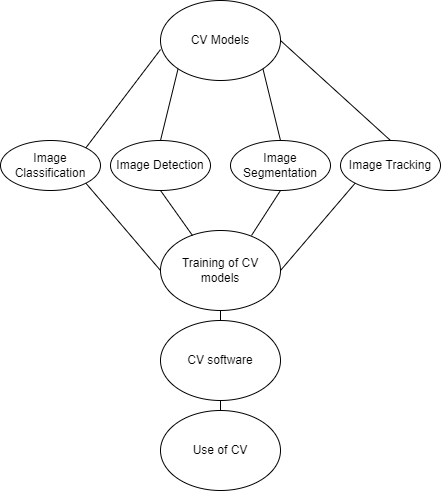
\includegraphics[scale=1.0]{diagram.pdf}
Aj text môže byť prezentovaný ako obrázok. Stane sa z neho označný plávajúci objekt. Po vytvorení diagramu zrušte znak \texttt{\%} pred príkazom \verb|\includegraphics| označte tento riadok ako komentár (tiež pomocou znaku \texttt{\%}).
\caption{Rozhodujúci argument.}
\label{f:rozhod}
\end{figure*}



\section{Výhody a nevýhody počítačoveho videnia} \label{ina}
Ako každa ina technologia aj počítačove videnie má svoje výhody a nevýhody.
\begin{itemize}
\item Porovnanie s ľudským videním
	\begin{itemize}
	\item ľudské videnie: zdroj obrazu → oko → kognitívny systém
	\item počítačové videnie: zdroj obrazu → kamera → počítač
	\end{itemize}
\end{itemize}

\begin{itemize}
\item Výhody
	\begin{enumerate}
	\item Uľahčuje množstvo procesov
	\item Úplné frekvenčné spekrum pre získanie obrazov
	\item Jednoduchý a rýchly spôsob získavania údajov
	\item Generovanie presných a presných údajov
	\item Finančne efektívne
	\end{enumerate}
\end{itemize}

\begin{itemize}
\item Nevýhody
	\begin{enumerate}
	\item Treba spravovávať veľmi velké množstvo informacií
	\item Citlivé na osvetlenie a rôzne iné javy
	\item Realny svet transformujeme 3D na 2D
	\item Je potrebné veľke množstvo pamäte
	\item Veľké množstvo nadbytočných údajov 
	\end{enumerate}
\end{itemize}


Základným problémom je teda\ldots{} Najprv sa pozrieme na nejaké vysvetlenie (časť~\ref{ina:nejake}), a potom na ešte nejaké (časť~\ref{ina:nejake}).\footnote{Niekedy môžete potrebovať aj poznámku pod čiarou.}

Môže sa zdať, že problém vlastne nejestvuje\cite{Coplien:MPD}, ale bolo dokázané, že to tak nie je~\cite{Czarnecki:Staged, Czarnecki:Progress}. Napriek tomu, aj dnes na webe narazíme na všelijaké pochybné názory%\cite{PLP-Framework}. Dôležité veci možno \emph{zdôrazniť kurzívou}.




\paragraph{Veľmi dôležitá poznámka.}
Niekedy je potrebné nadpisom označiť odsek. Text pokračuje hneď za nadpisom.


\section{Využiie počítačového videnia} \label{zaver} 


\section{Záver} \label{zaver} % prípadne iný variant názvu



%\acknowledgement{Ak niekomu chcete poďakovať\ldots}


% týmto sa generuje zoznam literatúry z obsahu súboru literatura.bib podľa toho, na čo sa v článku odkazujete
\bibliography{literatura}
\bibliographystyle{alpha} % prípadne alpha, abbrv alebo hociktorý iný
\end{document}
